% Póster A1 (594 x 841 mm, vertical) en inglés. Compilar con: tectonic poster_en.tex
\documentclass{article}
\usepackage[paperwidth=594mm,paperheight=841mm,margin=0mm]{geometry}
\usepackage{fontspec}
\setmainfont{texgyreheros}[Extension=.otf,UprightFont=*-regular,BoldFont=*-bold,ItalicFont=*-italic,BoldItalicFont=*-bolditalic]
\usepackage{xcolor,graphicx,tikz,tabularx,booktabs,qrcode,enumitem,array}
\usepackage[most]{tcolorbox}
\graphicspath{{fig/}{../}}

\definecolor{navy}{HTML}{0B2545}
\definecolor{teal}{HTML}{1B7F79}
\definecolor{amber}{HTML}{E0A100}
\definecolor{ink}{HTML}{1E2633}
\definecolor{paper}{HTML}{F6F4EE}
\definecolor{muted}{HTML}{5B6575}

\pagestyle{empty}
\setlength{\parindent}{0pt}
\setlength{\parskip}{0.55em}
\color{ink}

\newcommand{\body}{\fontsize{23}{30}\selectfont}
\newcommand{\figcap}[1]{\par\vspace{0.2em}{\fontsize{19}{24}\selectfont\color{muted}#1\par}}

% Encabezado de sección: número + título + filete
\newcommand{\sect}[2]{%
  \par\vspace{0.7em}%
  {\fontsize{34}{40}\selectfont\bfseries\color{teal}#1\hspace{0.4em}\color{navy}#2\par}%
  \vspace{0.15em}{\color{amber}\rule{\linewidth}{3pt}}\par\vspace{0.3em}}

% Cifra destacada
\newcommand{\kpi}[2]{%
  \begin{minipage}[t]{0.158\linewidth}\centering
    {\fontsize{56}{60}\selectfont\bfseries\color{amber}#1\par}\vspace{0.25em}
    {\fontsize{19}{23}\selectfont\color{white}#2\par}
  \end{minipage}}

\setlist[itemize]{leftmargin=1.1em,itemsep=0.25em,topsep=0.2em,label={\color{teal}\textbullet}}

\begin{document}
\pagecolor{paper}

% ---------------- Encabezado ----------------

\begin{tikzpicture}[remember picture,overlay]
  \fill[navy] (current page.north west) rectangle ([yshift=-150mm]current page.north east);
  \fill[amber] ([yshift=-150mm]current page.north west) rectangle ([yshift=-153mm]current page.north east);
  \fill[navy] (current page.south west) rectangle ([yshift=24mm]current page.south east);
\end{tikzpicture}

\vspace*{16mm}
\noindent\hspace*{24mm}\begin{minipage}[t]{546mm}
\begin{minipage}[t]{440mm}
  {\fontsize{24}{28}\selectfont\color{amber}\bfseries INTEGRATIVE PROJECT \,·\, DATA MINING \,·\, MACHINE LEARNING \,·\, CLOUD COMPUTING\par}
  \vspace{6mm}
  {\fontsize{84}{90}\selectfont\bfseries\color{white}TRM Predict\par}
  \vspace{3mm}
  {\fontsize{40}{48}\selectfont\color{white}A cloud-native predictive analytics system for\\ exchange-rate risk decisions in Colombia\par}
  \vspace{7mm}
  {\fontsize{27}{33}\selectfont\color{white}\bfseries Sebastián Cubides \quad Nicolás Vergara \quad Edgar Ruiz\par}
  \vspace{1mm}
  {\fontsize{23}{29}\selectfont\color{white!80!navy}Data Engineering and Artificial Intelligence, 5th semester \,·\, Universidad Santo Tomás, Tunja \,·\, 2026-2\par}
\end{minipage}%
\hfill
\begin{minipage}[t]{90mm}\centering
  \vspace{4mm}
  \colorbox{white}{\qrcode[height=62mm]{https://github.com/Sebas-409/proyecto-integrador-trm}}\par
  \vspace{3mm}
  {\fontsize{18}{22}\selectfont\color{white}Code, data and Terraform\par}
\end{minipage}

% ---------------- Cifras clave ----------------
\vspace{18mm}
\begin{tcolorbox}[enhanced,width=\linewidth,colback=navy,colframe=navy,arc=4mm,boxrule=0pt,
  left=6mm,right=6mm,top=7mm,bottom=7mm]
  \kpi{2,159}{trading days,\\ 43 leakage-free features}\hfill
  \kpi{19}{models tuned with\\ time-series CV}\hfill
  \kpi{0.586}{test ROC-AUC for\\ large-move risk}\hfill
  \kpi{+383}{COP/day per USD 1,000\\ for a remittance household}\hfill
  \kpi{100\%}{availability while\\ a server is killed}\hfill
  \kpi{+84\%}{throughput after\\ auto-scaling 2\,→\,4}
\end{tcolorbox}

% ---------------- Cuerpo en tres columnas ----------------
\vspace{2mm}
% ===== Columna 1 =====
\begin{minipage}[t]{174mm}\body

\sect{1}{The problem}
Colombian households received about \textbf{USD 11.8 billion} in remittances in 2024, and thousands of small importers pay in dollars. Both convert at the official exchange rate (\textbf{TRM}) without the analytics of large firms.

\textbf{Question:} can public market data say, one business day ahead, whether the TRM will rise and whether a large move is coming, and can that be served reliably and cheaply in the cloud?
\figcap{Aligned with SDG 8 (target 8.10, access to financial services) and SDG 10 (target 10.c, remittance costs).}

\sect{2}{Data and pipeline}
A CRISP-DM pipeline integrates four sources, refreshed every weekday by a serverless job:
\begin{itemize}
  \item Official TRM (datos.gov.co API, since 1991)
  \item 8 markets: Brent, DXY, US 10Y, VIX, S\&P 500, MXN, BRL, spot USD/COP (Yahoo)
  \item BTC and ETH daily candles (Binance)
  \item FX news sentiment, \textbf{web-scraped} from \emph{La República}
\end{itemize}
A strict as-of join uses only market closes \emph{before} each TRM date, so no future information leaks into the features.

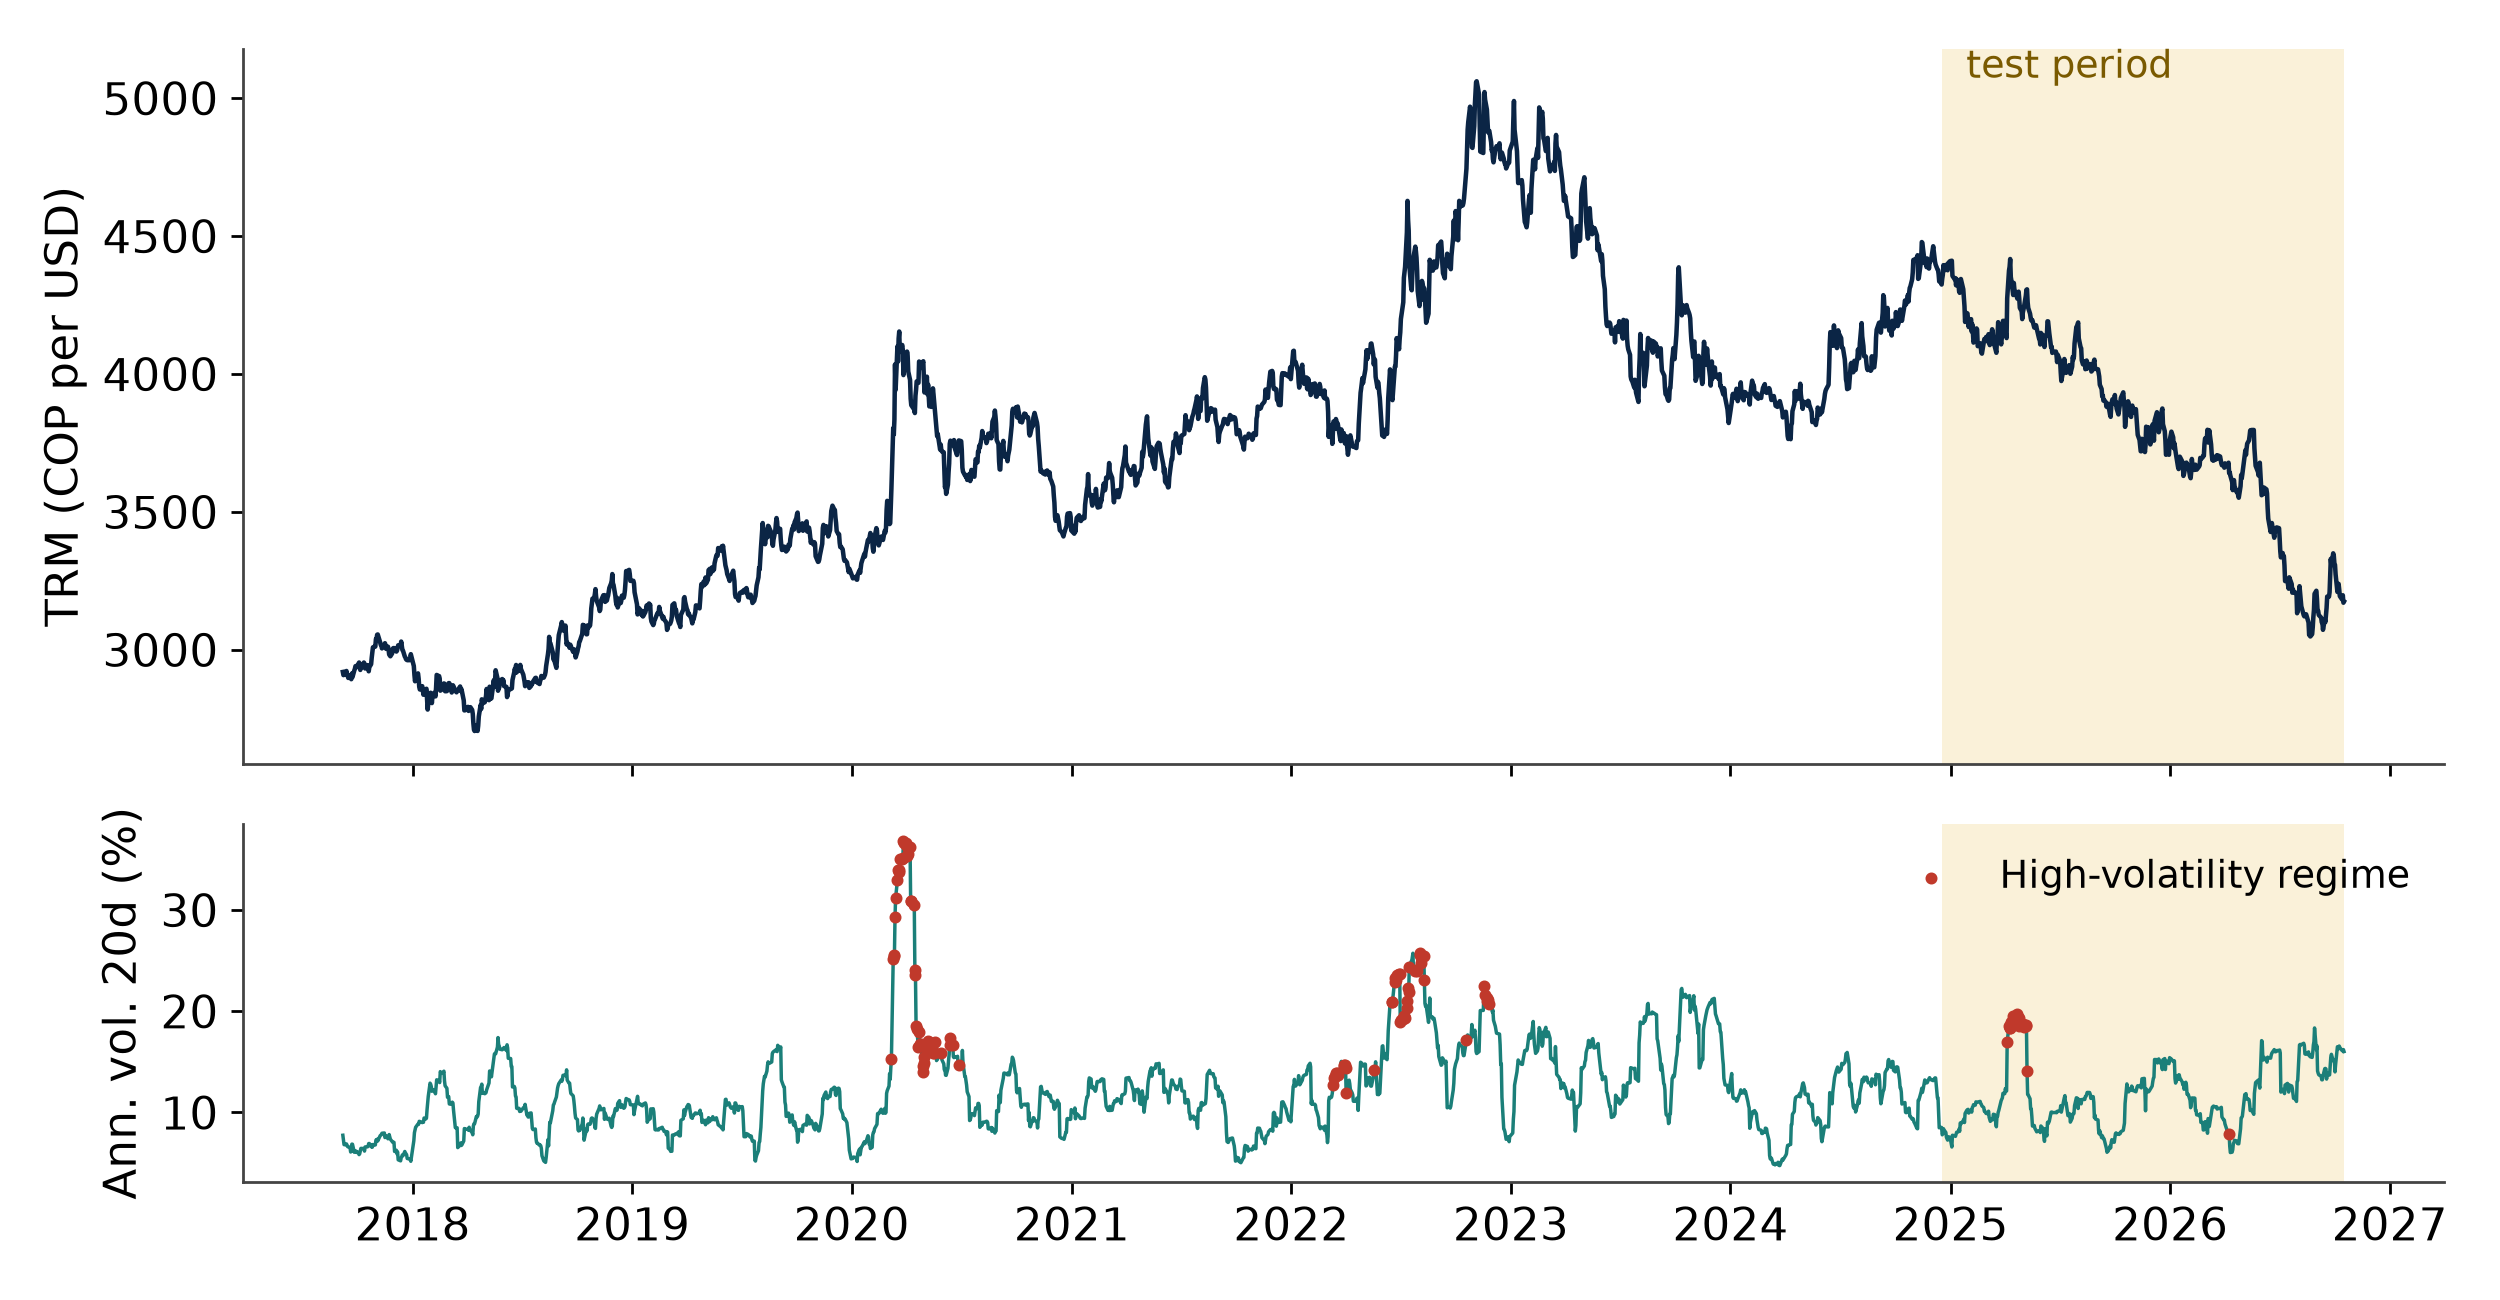
\includegraphics[width=\linewidth]{trm_series.png}
\figcap{TRM and 20-day volatility, Sep. 2017 to Oct. 2026. Red: days in the high-volatility regime found by clustering. Shaded: the 432 test days, never used for training.}

\sect{3}{Data mining}
\begin{itemize}
  \item \textbf{PCA + K-Means / Ward:} 3 market regimes. In risk-off days the TRM rises next day 52.9\% of the time; in risk-on days, 44.3\%.
  \item \textbf{DBSCAN} flags \textbf{57 anomalous days} (45 in 2020), with 1.7$\times$ the normal next-day volatility.
  \item \textbf{Apriori = FP-Growth:} 91 rules, e.g.\\ \emph{BRL up \& MXN up \& VIX up $\Rightarrow$ TRM up} (confidence 0.60, lift 1.24).
\end{itemize}
\end{minipage}%
\hspace{12mm}%
% ===== Columna 2 =====
\begin{minipage}[t]{174mm}\body

\sect{4}{Machine learning}
Three tasks for the next business day: \textbf{direction} (up/down), \textbf{risk} (move larger than the 75th percentile, 0.86\%) and \textbf{return} (regression). 19 models were tuned with Grid/Random Search inside a 5-fold \texttt{TimeSeriesSplit} and chosen by CV score only.

\centerline{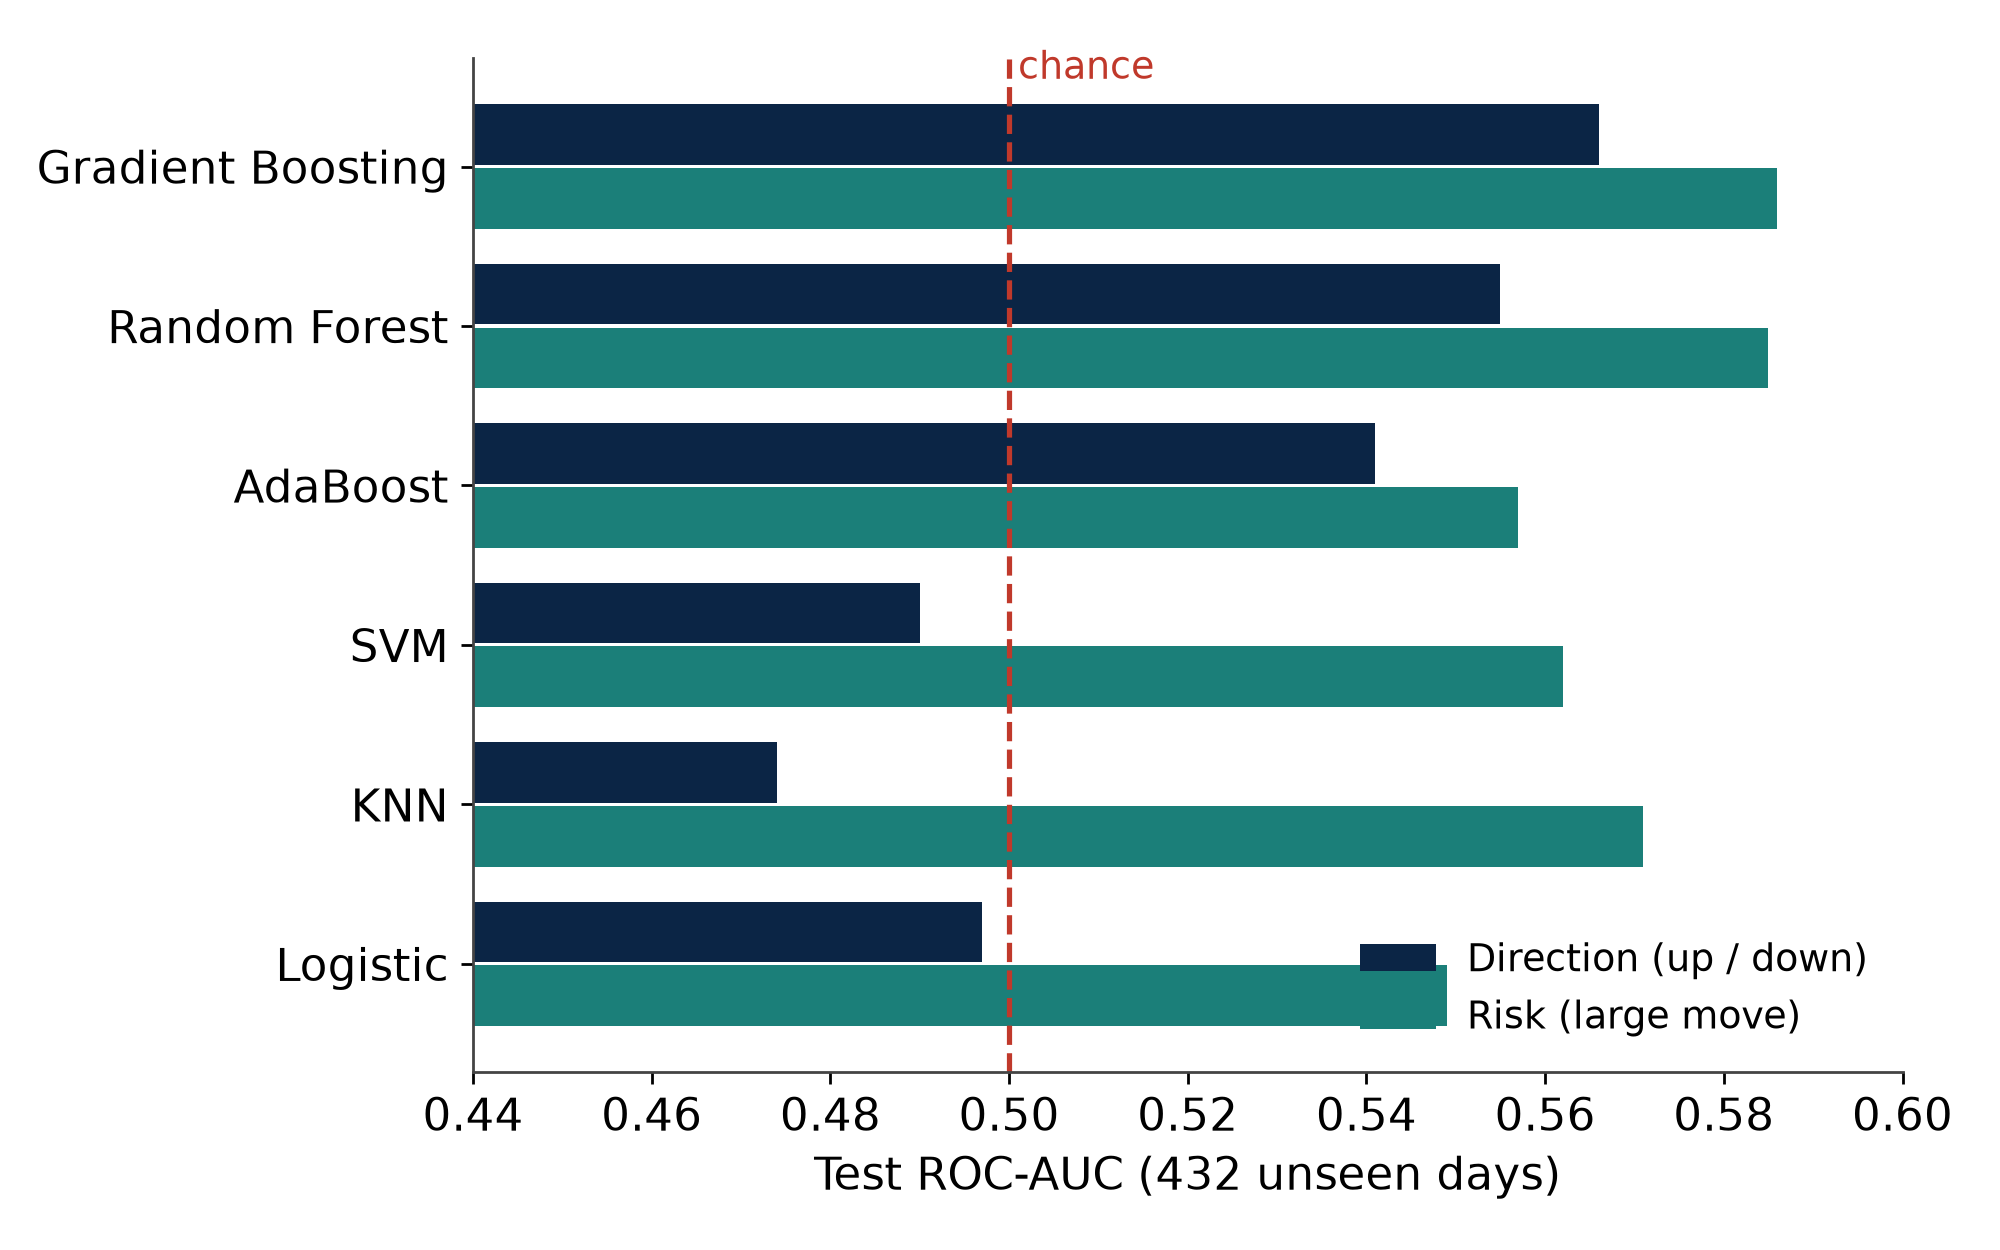
\includegraphics[width=0.9\linewidth]{model_auc.png}}
\figcap{Out-of-sample ROC-AUC. Linear, KNN and SVM models fall to chance; only tree ensembles keep a signal.}

\begin{itemize}
  \item Regression: Gradient Boosting RMSE \textbf{2.4\% below the random walk}; Random Forest gets the sign right 54.6\% of the time.
  \item Selected: \textbf{Random Forest} for all three tasks (best CV in 2 of 3, one family to maintain).
\end{itemize}

\sect{5}{Why the model decides}
\centerline{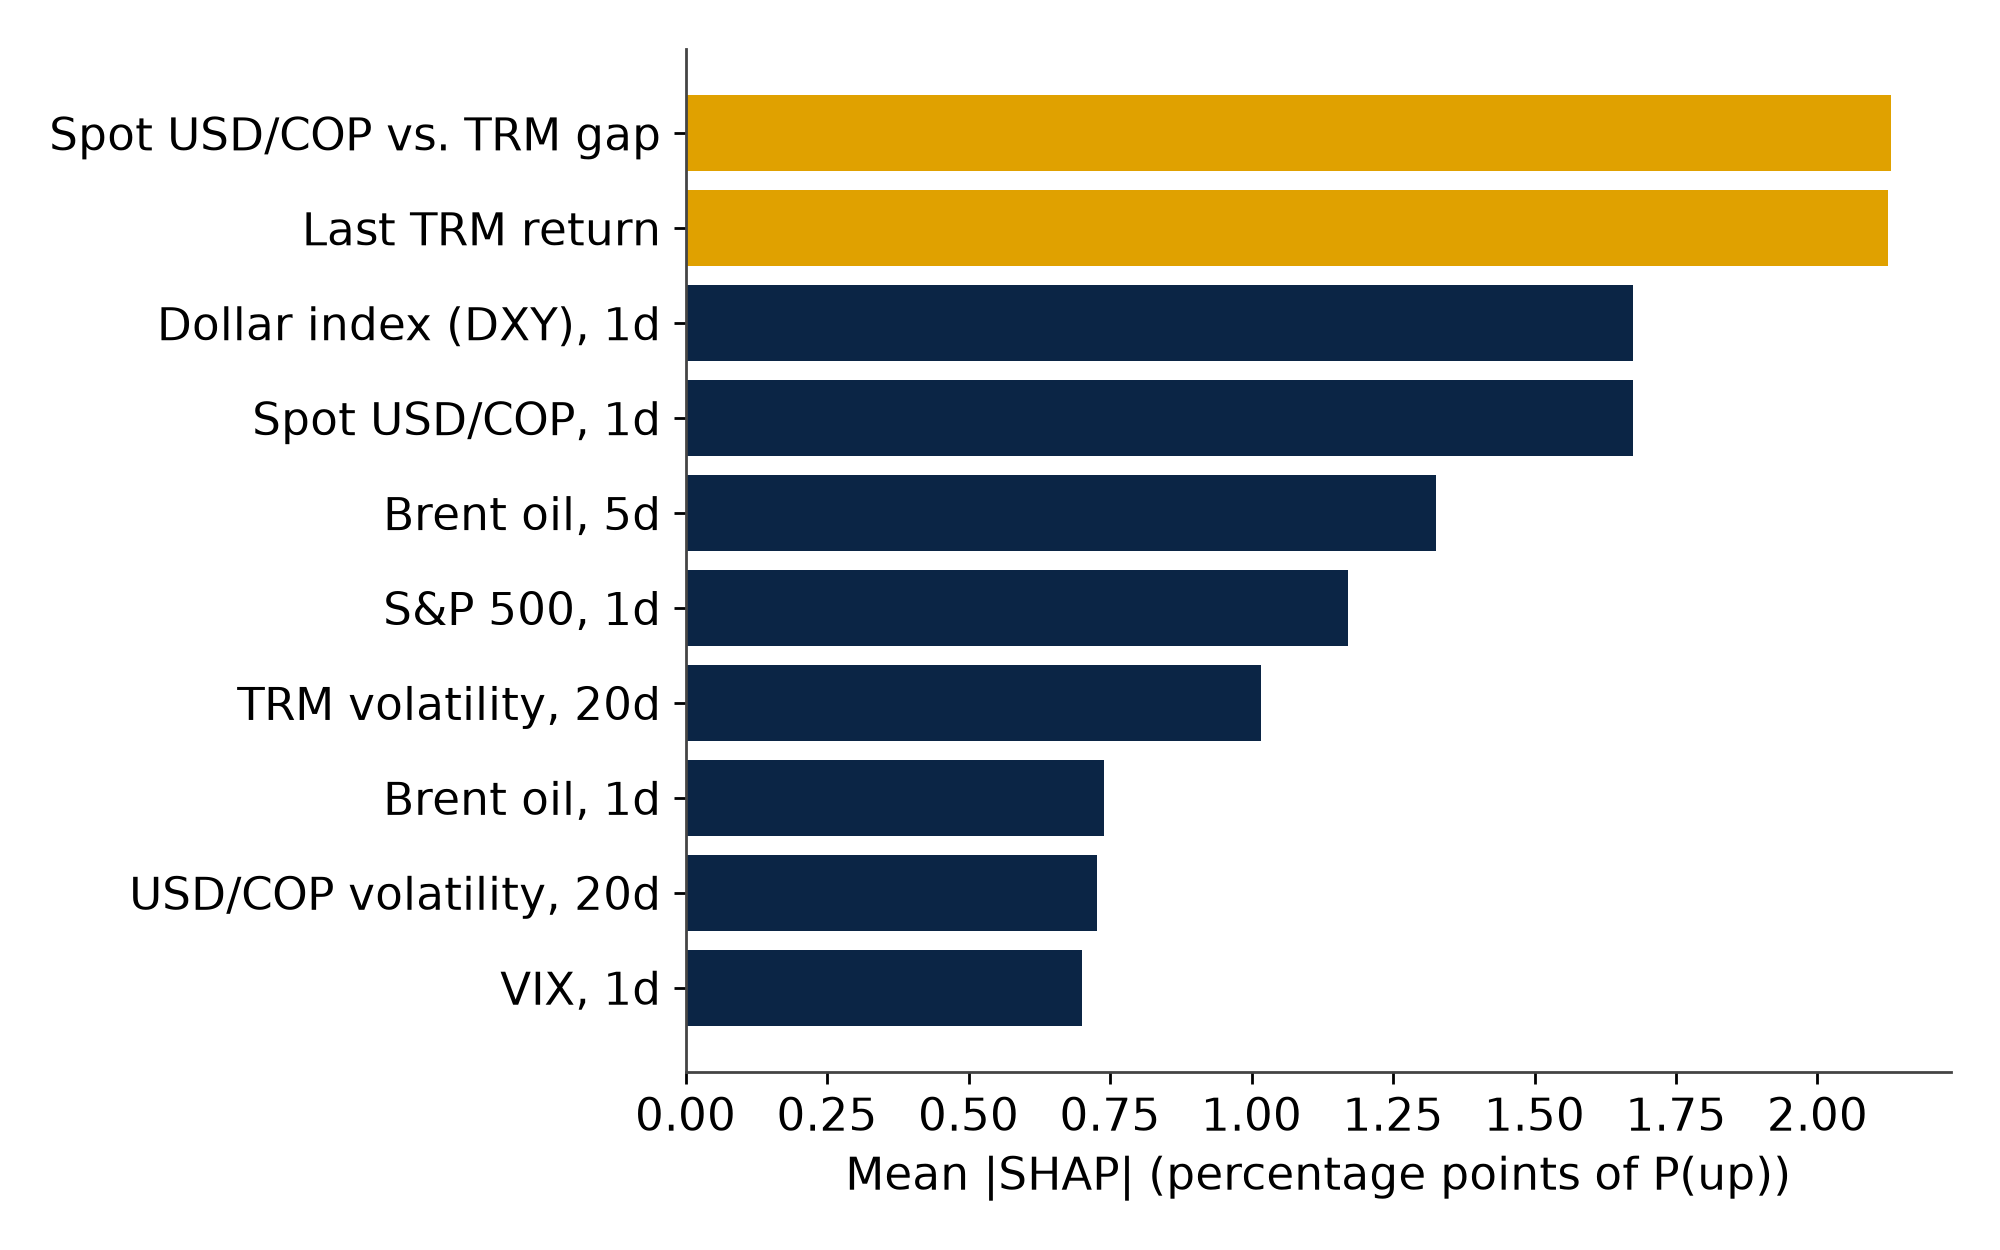
\includegraphics[width=0.9\linewidth]{shap_top10.png}}
\figcap{TreeSHAP importance. The engineered spot--TRM gap ranks first: the TRM averages the day's trades, so a spot quote above it anticipates a rise.}

\sect{6}{Does it help a user?}
A household receiving USD 1,000 a day sells at once, or waits one day when $P(\text{up})>0.5$.
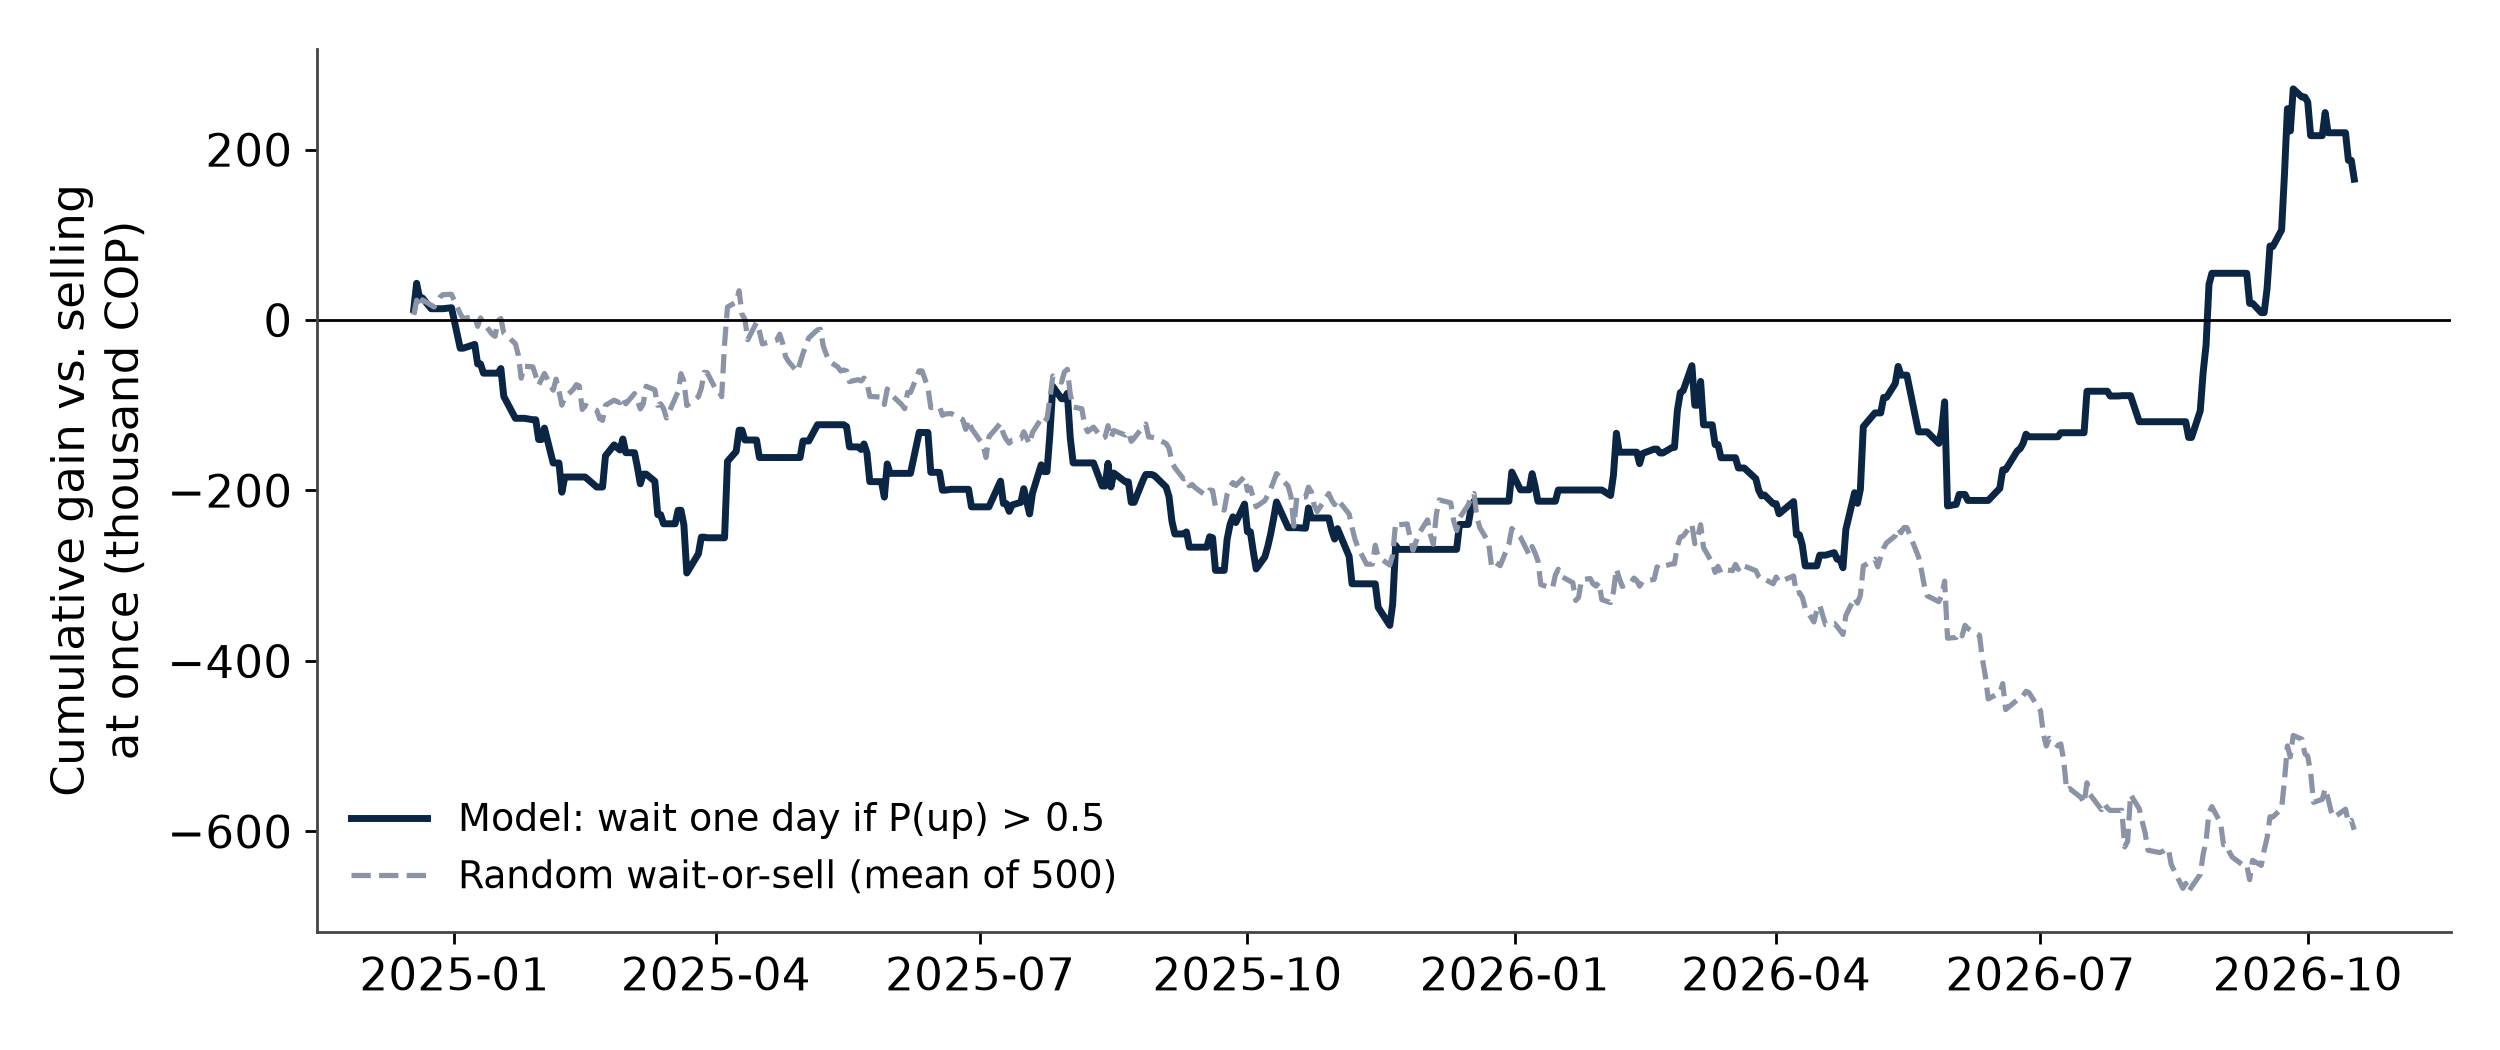
\includegraphics[width=\linewidth]{backtest.png}
\figcap{Test period. Model: +383 COP/day (+624 with threshold 0.55). Random choice: $-$1,383 COP/day. The risk alert has 30.1\% precision vs.\ a 22.5\% base rate (lift 1.34).}
\end{minipage}%
\hspace{12mm}%
% ===== Columna 3 =====
\begin{minipage}[t]{174mm}\body

\sect{7}{Architecture on AWS}
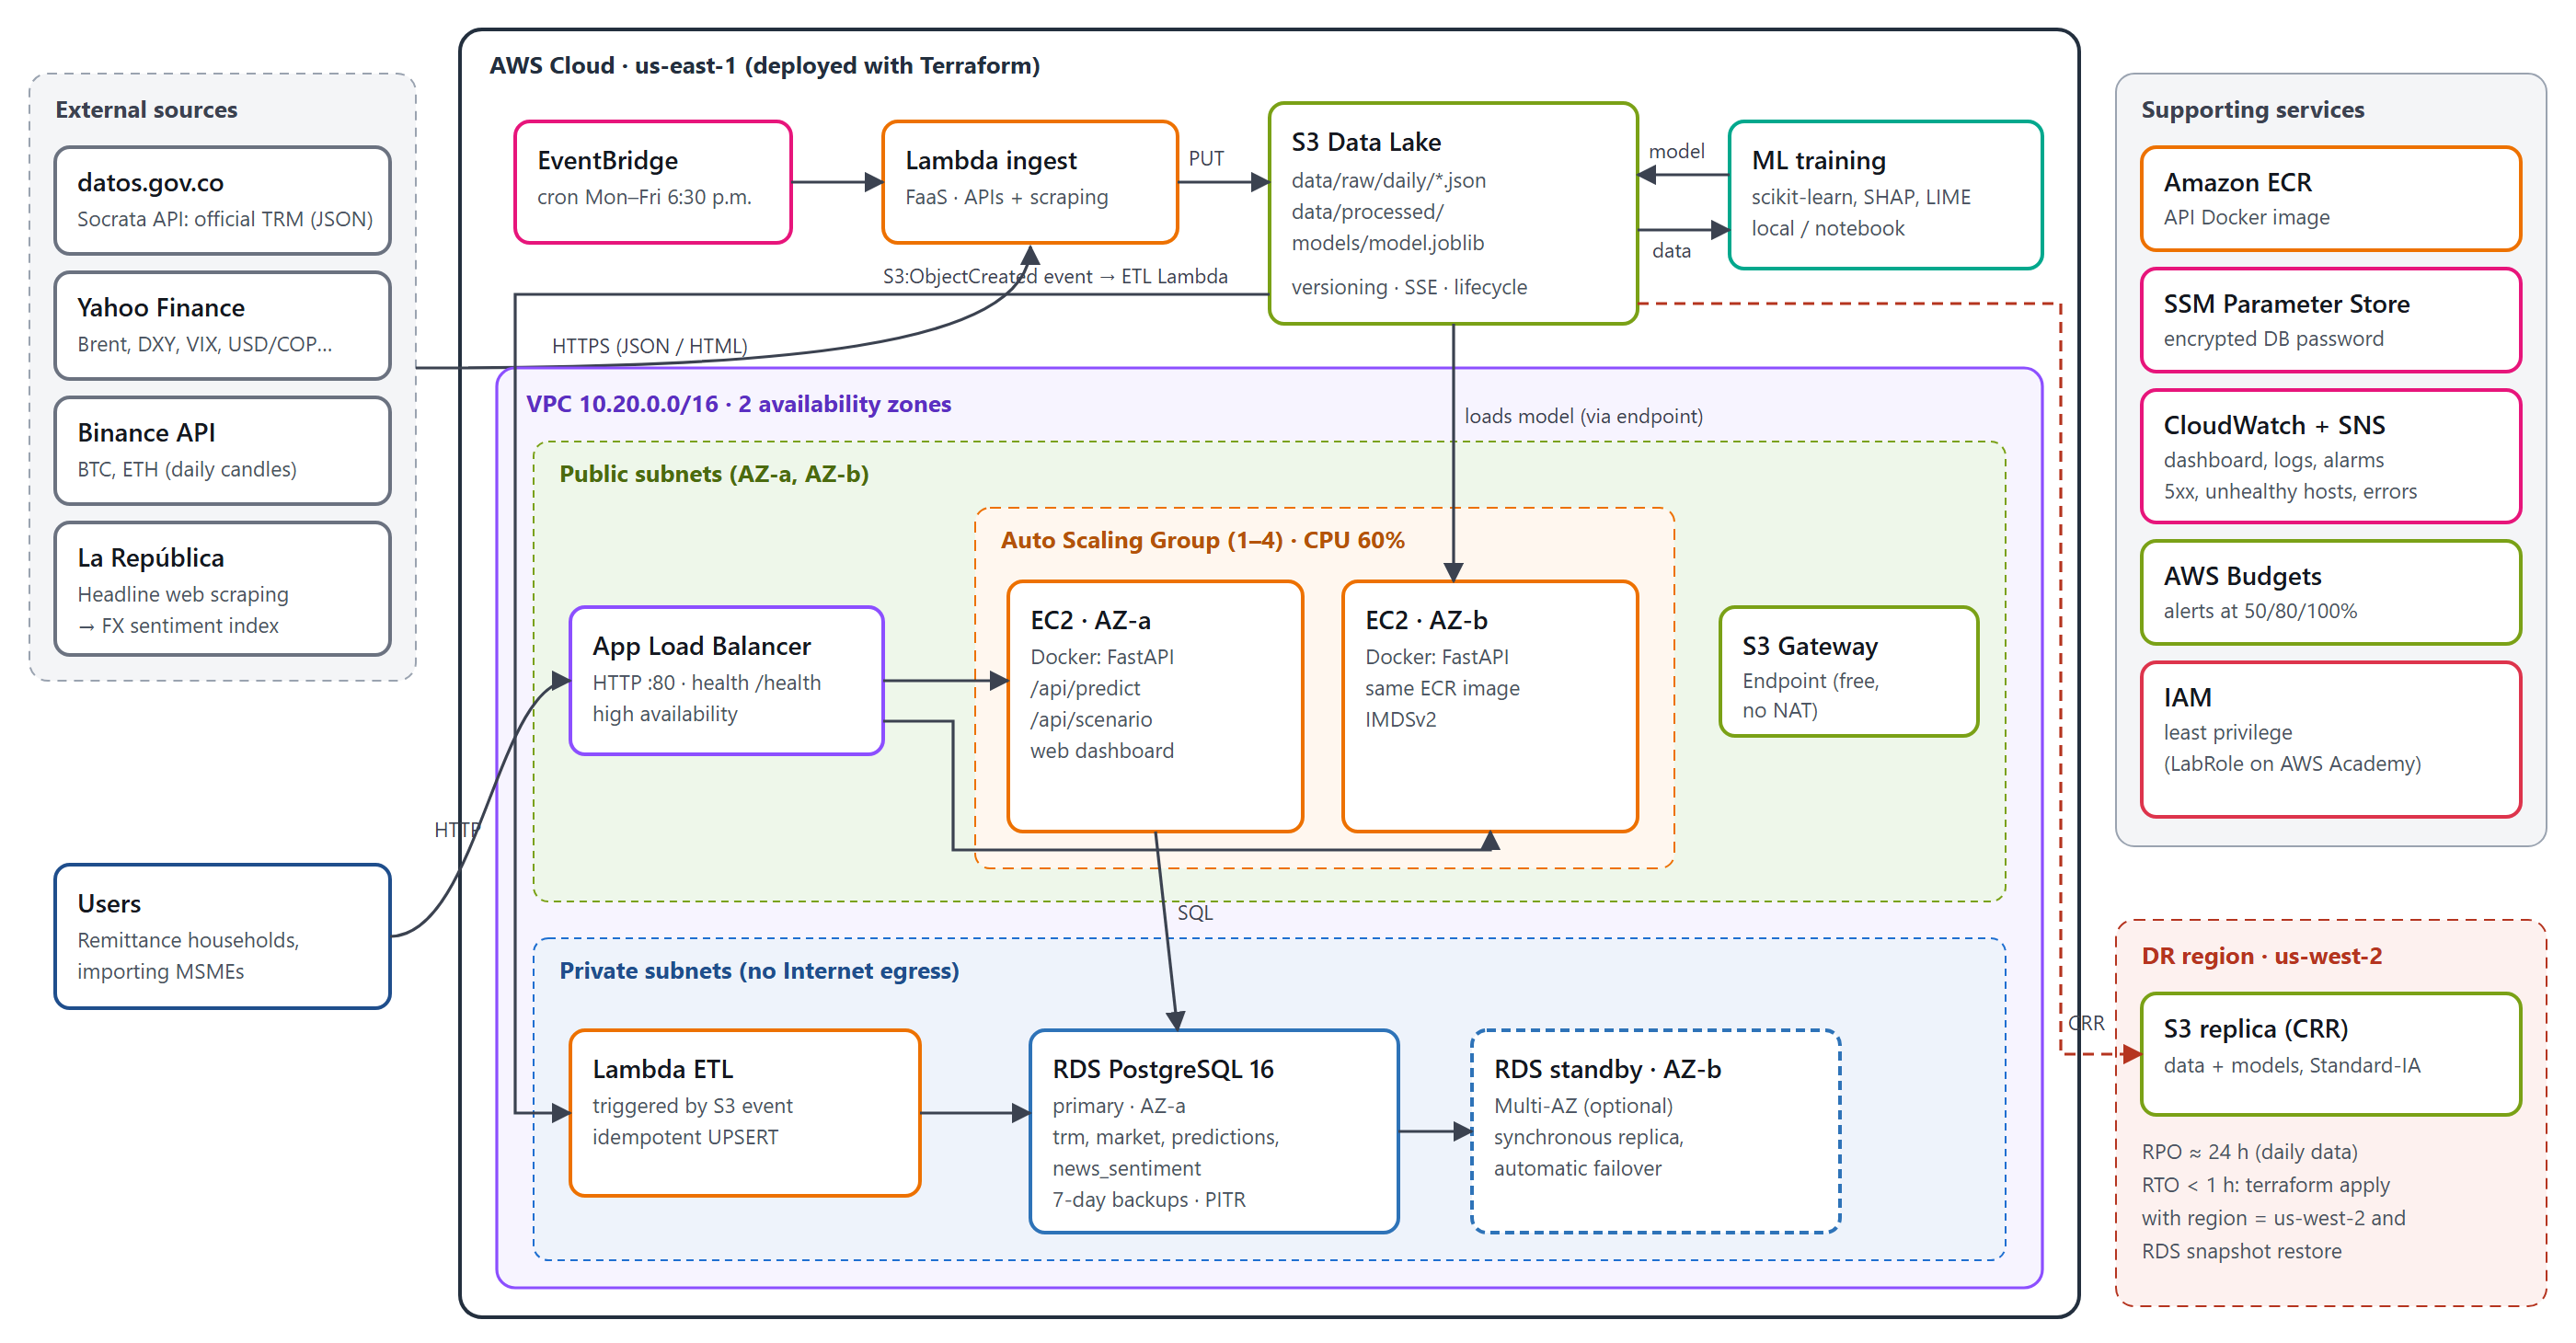
\includegraphics[width=\linewidth]{arquitectura_en.png}
\figcap{64 resources in Terraform. Lambda ingestion and ETL, S3 data lake replicated to us-west-2, RDS PostgreSQL, and a Docker FastAPI behind an ALB with an Auto Scaling group across two availability zones.}

\sect{8}{Cloud experiments}
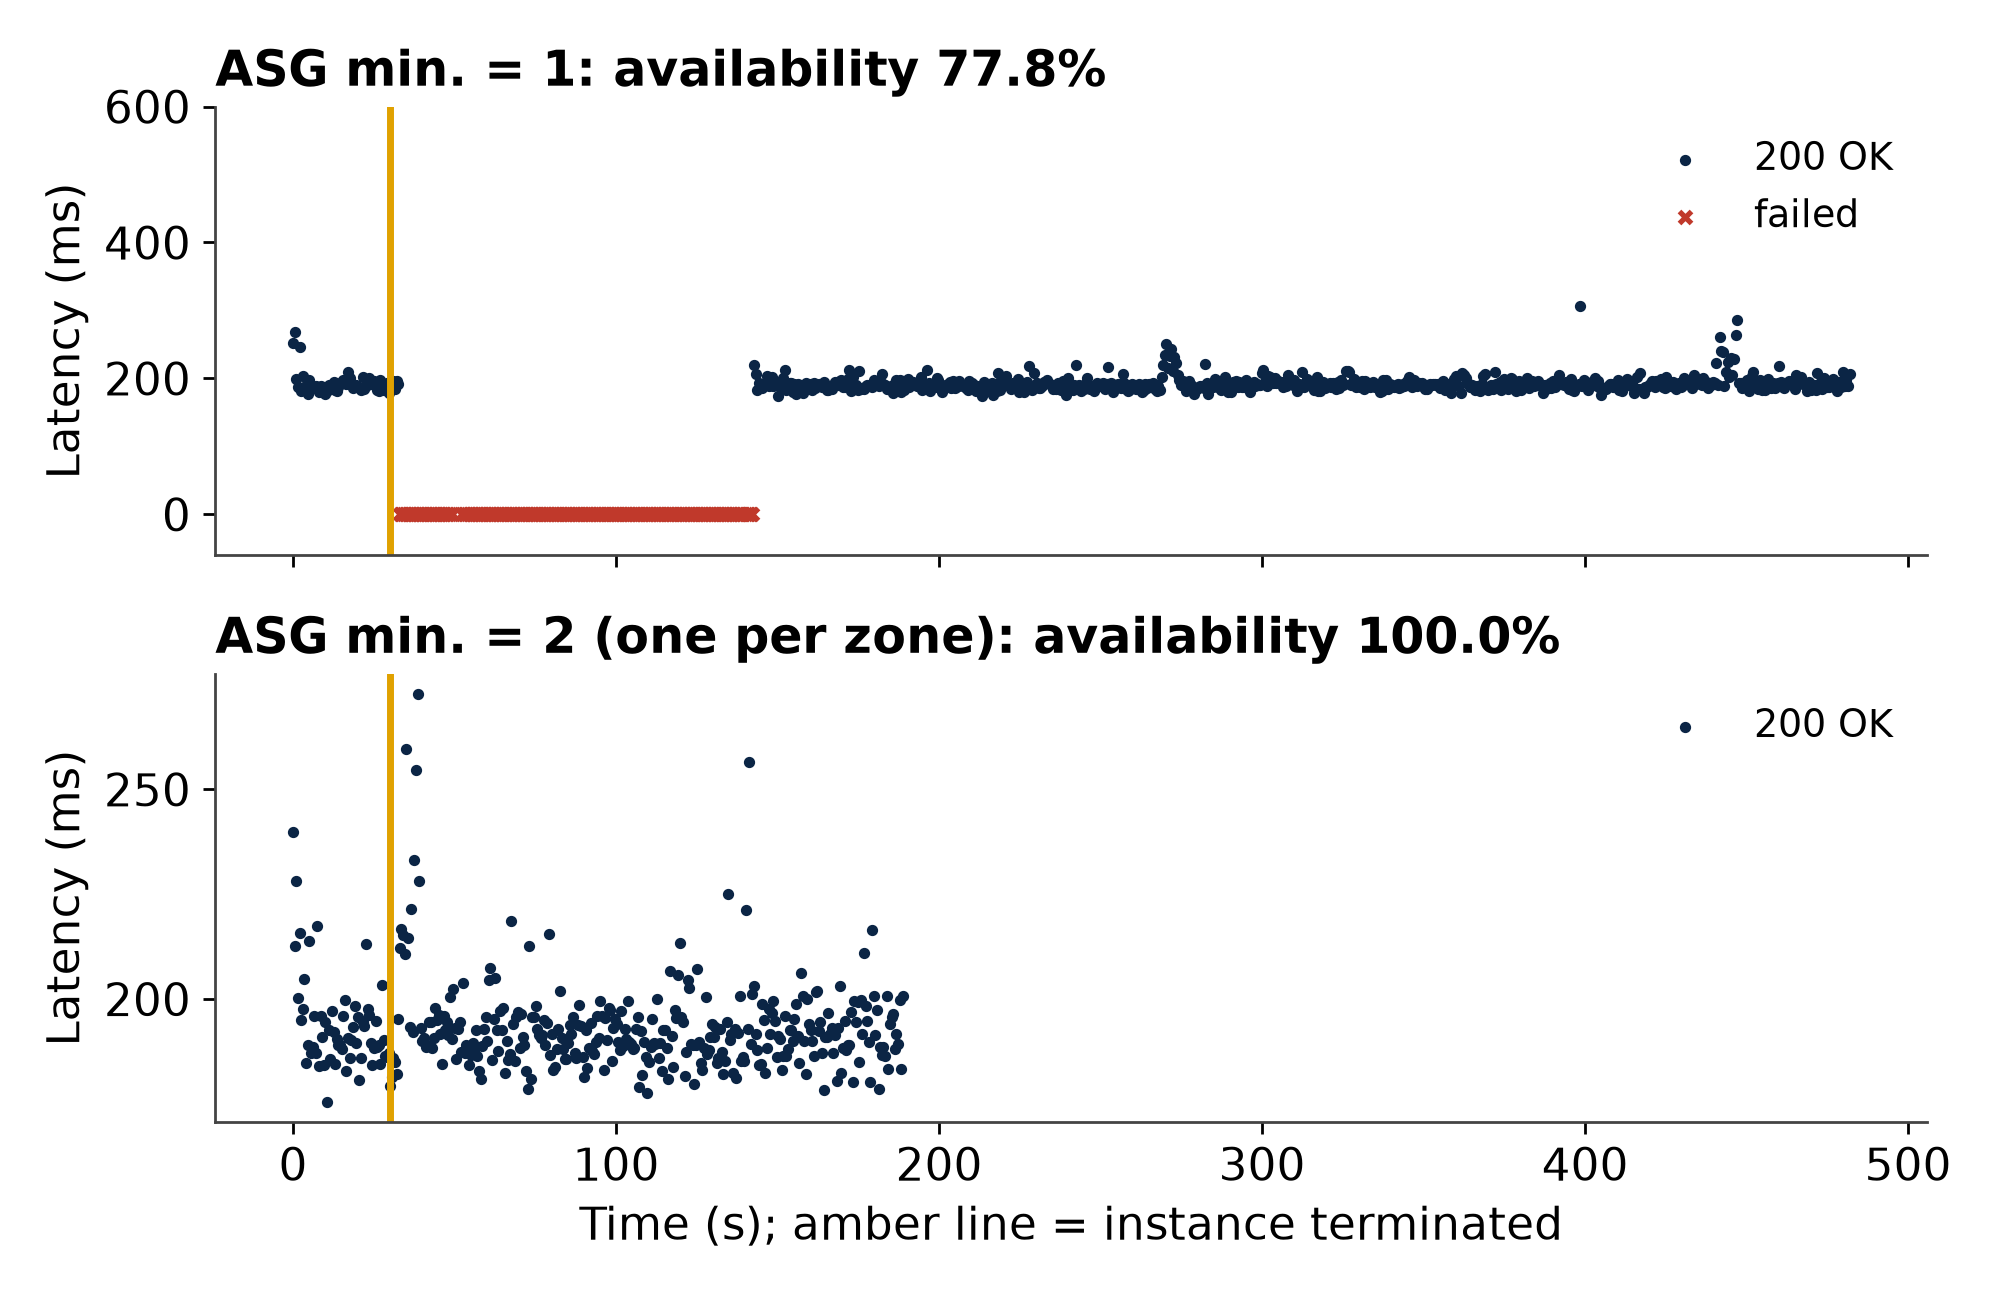
\includegraphics[width=\linewidth]{ha_poster.png}
\figcap{One instance terminated at $t=30$\,s. With an ASG minimum of 1 the site was down for 109\,s; with one instance per zone, \textbf{0 of 378} requests failed.}

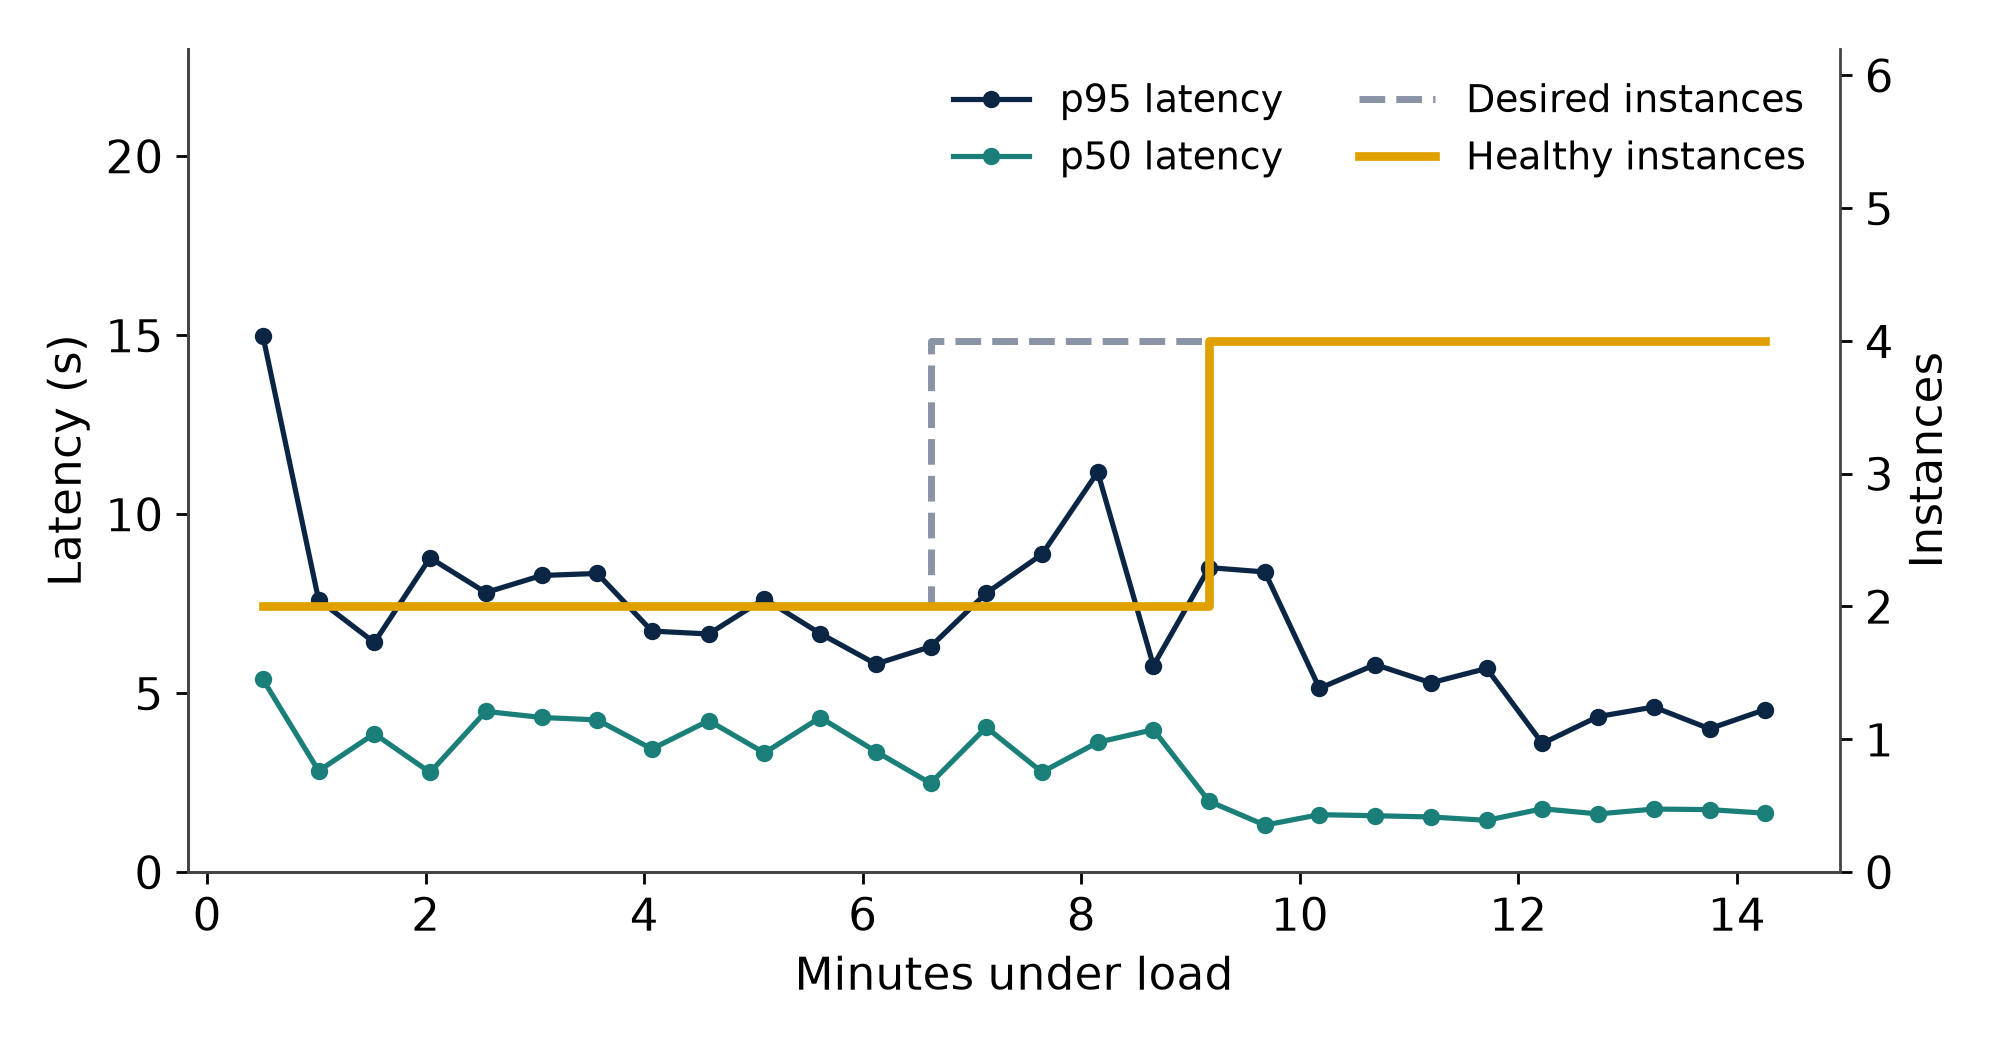
\includegraphics[width=\linewidth]{load_poster.png}
\figcap{16 concurrent clients for 14 min. Target tracking at 60\% CPU scales 2\,→\,4: 4.1\,→\,7.6 req/s, median latency 4.0\,→\,1.6\,s, \textbf{0 errors in 4,543} requests.}

\sect{9}{Cost and conclusions}
About \textbf{USD 64/month} on demand (ALB, EC2, public IPv4 and RDS dominate); no NAT gateway saves USD 33. Created and destroyed with Terraform, the whole semester costs about \textbf{USD 21}.
\begin{itemize}
  \item Daily FX is hard to predict, but a small, honest edge can still beat random decisions.
  \item High availability needs the right \emph{scaling policy}, not only two zones.
\end{itemize}
\end{minipage}
\end{minipage}

% ---------------- Pie ----------------
\begin{tikzpicture}[remember picture,overlay]
  \node[anchor=west,text=white,font=\fontsize{18}{22}\selectfont] at ([xshift=24mm,yshift=12mm]current page.south west)
    {References: Meese \& Rogoff (1983) \,·\, Breiman (2001) \,·\, Friedman (2001) \,·\, Lundberg \& Lee (2017) \,·\, Ester et al. (1996) \,·\, Agrawal \& Srikant (1994)};
\end{tikzpicture}
\end{document}
